% Updated in September 2014 by Hideo Saito
% Updated in September 2012 by In Kyu Park
% Updated in April 2002 by Antje Endemann, ...., and in September 2010 by Reinhard Klette
% Based on CVPR 07 and LNCS style, with modifications by DAF, AZ and elle 2008, AA 2010, ACCV 2010, ACCV 2012

\documentclass[runningheads]{llncs}
\usepackage{graphicx}
\usepackage{amsmath,amssymb} % define this before the line numbering.
%\usepackage{lineno}
\usepackage{color}
\usepackage{cite}

%===========================================================
\begin{document}

%macro for raising the point in decimal numbers; see example in the abstract
\newcommand{\point}{
    \raise0.7ex\hbox{.}
    }

%Do   -- NOT --    use any additional macros

\pagestyle{headings}

\mainmatter

%===========================================================
\title{Camera Movement and Surrounding Scene Appearance as Contextual Features for Action Recognition} % Replace with your title

\titlerunning{Camera Movement and Surrounding Scene Appearance as Contextual Features for Action Recognition} % Replace with your title

\authorrunning{Fabian Caba Heilbron, Ali Thabet, Juan Carlos Niebles and Bernard Ghanem} % Replace with your names

\author{Fabian Caba Heilbron\textsuperscript{1,2}, Ali Thabet\textsuperscript{1}, Juan Carlos Niebles\textsuperscript{2} and Bernard Ghanem\textsuperscript{1}} % Replace with your names
\institute{King Abdullah University of Science and Technology (KAUST), Thuwal, Saudi Arabia\textsuperscript{1}\\
Universidad del Norte, Barranquilla, Colombia\textsuperscript{2}} % Replace with your institute's address

\maketitle

%===========================================================
\begin{abstract}
This paper describes a framework for recognizing human actions in videos by incorporating a new set of visual cues that represent the \emph{context} of the action. We develop a weak foreground-background segmentation approach in order to robustly extract not only foreground features that are focused on the actors, but also global camera motion and contextual scene information. Using dense point trajectories, our approach separates and describes the foreground motion from the background, represents the appearance of the extracted static background, and encodes the global camera motion that interestingly is shown to be discriminative for certain action classes. Our experiments on four challenging benchmarks (HMDB51, Hollywood2, Olympic Sports, UCF50) show that our contextual features enable a significant performance improvement over state-of-the-art algorithms.
\end{abstract}

%===========================================================
\section{Introduction} \label{introduction}

Human action recognition is a challenging task for computer vision algorithms due to the large variabilities in video data caused by occlusions, camera motions, actor and scene appearances, among others. A popular current trend in action recognition methods relies on using local video descriptors to represent visual events in videos \cite{laptev2005, dollar2005, wang2011}. These features are usually aggregated into a compact representation, namely the bag-of-features (BoF) representation \cite{laptev2008}. The advantage of this simple representation is that it avoids difficult pre-processing steps such as motion segmentation and tracking. In the BoF representation, local descriptors are quantized using a pre-computed codebook of visual patterns. This representation combined with discriminative classifiers such as support vector machines (SVM), has been quite successful in recognizing human actions  in controlled scenarios \cite{blank2005, schuldt2004}. Due to its simplicity, BoF requires the use of strong, robust and informative features, which can be obtained reliably in such simplified scenarios.

% Figure 1.
\begin{figure*}[ht]
\begin{center}
%\fbox{\rule{0pt}{1in} \rule{0.9\linewidth}{0pt}}
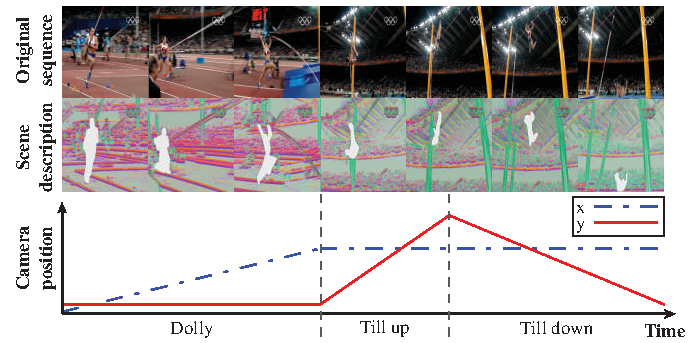
\includegraphics[width=0.98\linewidth]{pull_figure.pdf}
\end{center}
\caption{Some human actions have important correlations with surrounding cues. As observed in the first row, there is a video sequence associated with the human action pole vault. It is also noticeable that the camera moves according to some specific patron for capturing the movement of the subject. Specifically, the camera moves within dolly panning tracking when the athlete is approaching the plant and take off. Then, camera slightly starts to tilling up and tilling down when the person is flying away and falling respectively. Additionally, a better description can be performed if visual appearance of the track field is captured.}
\label{fig:pull_figure}
\end{figure*}

However, recent efforts have been made to collect more realistic video datasets (\emph{e.g.} from movies and personal videos uploaded to video sharing websites  \cite{kuehne2011,  marszalek2009}), which are useful for evaluating human action recognition methods in more natural settings. In fact, these datasets represent a challenge for existing BoF-based methods due to dynamic backgrounds, variations in illumination and viewpoint, and camera motion among other visual nuisances that can severely affect recognition performance. To mitigate the effect of camera motion in describing the action of interest in a video, recent methods \cite{wang2013,wang2011} have proposed using dense point trajectories in a video. In fact, these trajectories can separate background from foreground using a simple camera motion model (\emph{i.e.} an affine or homography transform between consecutive frames). Such separation allows action recognition approaches to robustly extract and describe foreground motion, which is otherwise contaminated by camera motion and the background. Inspired by this work, our proposed method also makes use of these dense trajectories; however, we enlist a more general camera model (by estimating the fundamental matrix between consecutive video frames) that allows for a more reliable separation between foreground and background pixels, especially in non-planar cluttered scenes. Unlike most other methods, we claim that the \emph{context} of a human action, namely global camera motion and static background appearance, can also be used to discriminate between certain human actions. These cues can also be considered as contextual features for an action, which would allow classification algorithms to mine the relationship between the human action and both the background scene as well as the camera motion. The appearance of the scene in which an action occurs can be helpful in recognizing the action, as validated by previous work in \cite{marszalek2009}. For example, a `cooking' action tends to occur indoors, while a `jogging' action usually exists outdoors. Interestingly, the manner in which the \emph{cameraman} records a particular action can also be indicative of the action. For example, camera zoom with minimal panning usually indicates an action that is spatially limited to a smaller physical space (\emph{e.g.} juggling balls), while significant panning is indicative of actions that require a much larger spatial support (\emph{e.g.} practicing long jump). Our proposed approach mines these two sources of contextual information, as well as, the separated foreground motion to describe and recognize an action. Figure \ref{fig:pull_figure} illustrates our claims.

%-------------------------------------------------------------------------
% Related work
\subsection*{Related work}\label{subsec: related work}
A large body of work has studied the problem of human action recognition in video. For a survey of this work, we refer the reader to \cite{aggarwal2011}. In this section, we give an overview of previous work that is most relevant to our proposed method.

\paragraph{\textbf{Action Recognition Pipeline.}} The majority of action recognition methods rely on local descriptors to represent visual events in videos \cite{laptev2005,dollar2005,wang2011}. Traditionally, these features are usually aggregated into a compact representation using the bag-of-features (BoF) framework \cite{laptev2008, escorcia2013}. Moreover, recent studies show that using soft encoding techniques, such as  Fisher Vectors \cite{perronnin2010} and Vectors of Locally Aggregated Descriptors (VLAD) \cite{jegou2012}, can lead to a boost in action recognition performance. These representations combined with discriminative classifiers such as support vector machines (SVM), have been quite successful in discriminating human action classes. However, as discussed in \cite{xwang2013}, there remain many details of the overall action recognition pipeline that can be extensively explored, including feature extraction, feature pre-procesing, codebook generation, feature encoding and pooling and normalization. In this paper, we propose a new set of features that can be used to address some of the limitations of conventional feature extraction methods.

\paragraph{\textbf{Feature Extraction.}} When applied to videos with substantial camera motion, traditional feature extraction approaches \cite{dollar2005, laptev2005} tend to generate a large number of features, which are inherently dependent on the camera motion in a video, thus, limiting their discriminative power among action classes. In order to overcome this issue, Wu \emph{et al.} \cite{wu2011} propose the use of Lagrangian point trajectories for action description in videos acquired with moving cameras. Their method compensates for global camera motion and only extracts features that exhibit motion independent of the camera movement, thus, outperforming traditional feature extraction algorithms. Park \emph{et al.} \cite{park2013} use a weak video stabilization method based on extracting coarse optical flow to isolate limb motion while canceling pedestrian translation and camera motion. Wang \emph{et al.} \cite{wang2011} present a method for action recognition using dense sampling of point trajectories. Their method handles large camera motions by limiting the maximum length of tracked trajectories. Despite their simplicity, these dense trajectory features have been shown to achieve a significant performance improvement as compared to conventional detection of sparse and salient spatiotemporal features \cite{laptev2005}.

More recent methods improve upon the aforementioned dense trajectory features. For example, Jain \emph{et al.} \cite{jain2013} propose a method to estimate more reliable trajectory features for action recognition. This method provides additional reliability and robustness to the feature extraction stage by initially decomposing optical flow into dominant and residual motions. Dominant motion is estimated using an affine frame-to-frame motion model and is subtracted from the computed optical flow to obtain the residual motion, which is attributed to the human action of interest. Similarly, `improved trajectories' are proposed in \cite{wang2013} to stabilize features and compensate for simple camera motion. This is done by fitting a frame-to-frame homography (using RANSAC) to separate moving points of the human action from those of the background. By explicitly canceling out the camera motion, their framework improves the performance of several motion descriptors, including trajectory shape, histogram of optical flow (HOF), and motion boundary histograms (MBH). While these methods have been successful in separating background/residual motions, contextual cues of human actions are usually discarded, thus, ignoring relevant information such as the static scene appearance and distinct camera motions correlated with specific actions.

Moreover, a few approaches have investigated ways to involve background scene information in the action recognition pipeline. Marszalek \emph{et al.} \cite{marszalek2009} incorporate context information from movie scripts by modeling the relationship between human actions and static scenes based on textual co-occurrence. While such textual co-occurrence helps recognition, they are restricted only to video sources where scripts are available. In \cite{ikizler2010}, multiple feature channels are integrated from different sources of information including human motion, scene information, and objects in the scene. However, this approach makes use of all pixels (corresponding to both the human action and background scene) to generate a global descriptor of the static scene \cite{oliva2001}. Rather than computing such a holistic representation, our proposed method separately computes a scene descriptor only from the extracted background, a motion descriptor from the extracted foreground trajectories, and a camera motion descriptor from the estimated transformations between consecutive frames.

In this paper, our goal is to reliably alleviate the effect of camera motion, as well as, incorporate features describing the surrounding of an action to build a richer representation for human actions. We are motivated by the fact that most videos are filmed with an intention and therefore there exists a correlation between the inherent camera motion in a video and the portrayed human action itself. We encode this intention with a weak camera motion model based on frame-to-frame fundamental matrices in a video. To the best of our knowledge, this is the first work to mine such a relationship between human actions and the filming process.

%===========================================================
\section{Proposed Methodology} \label{methodology}

% Figure 2
\begin{figure*}[t!]
\begin{center}
%\fbox{\rule{0pt}{3in} \rule{0.9\linewidth}{0pt}}
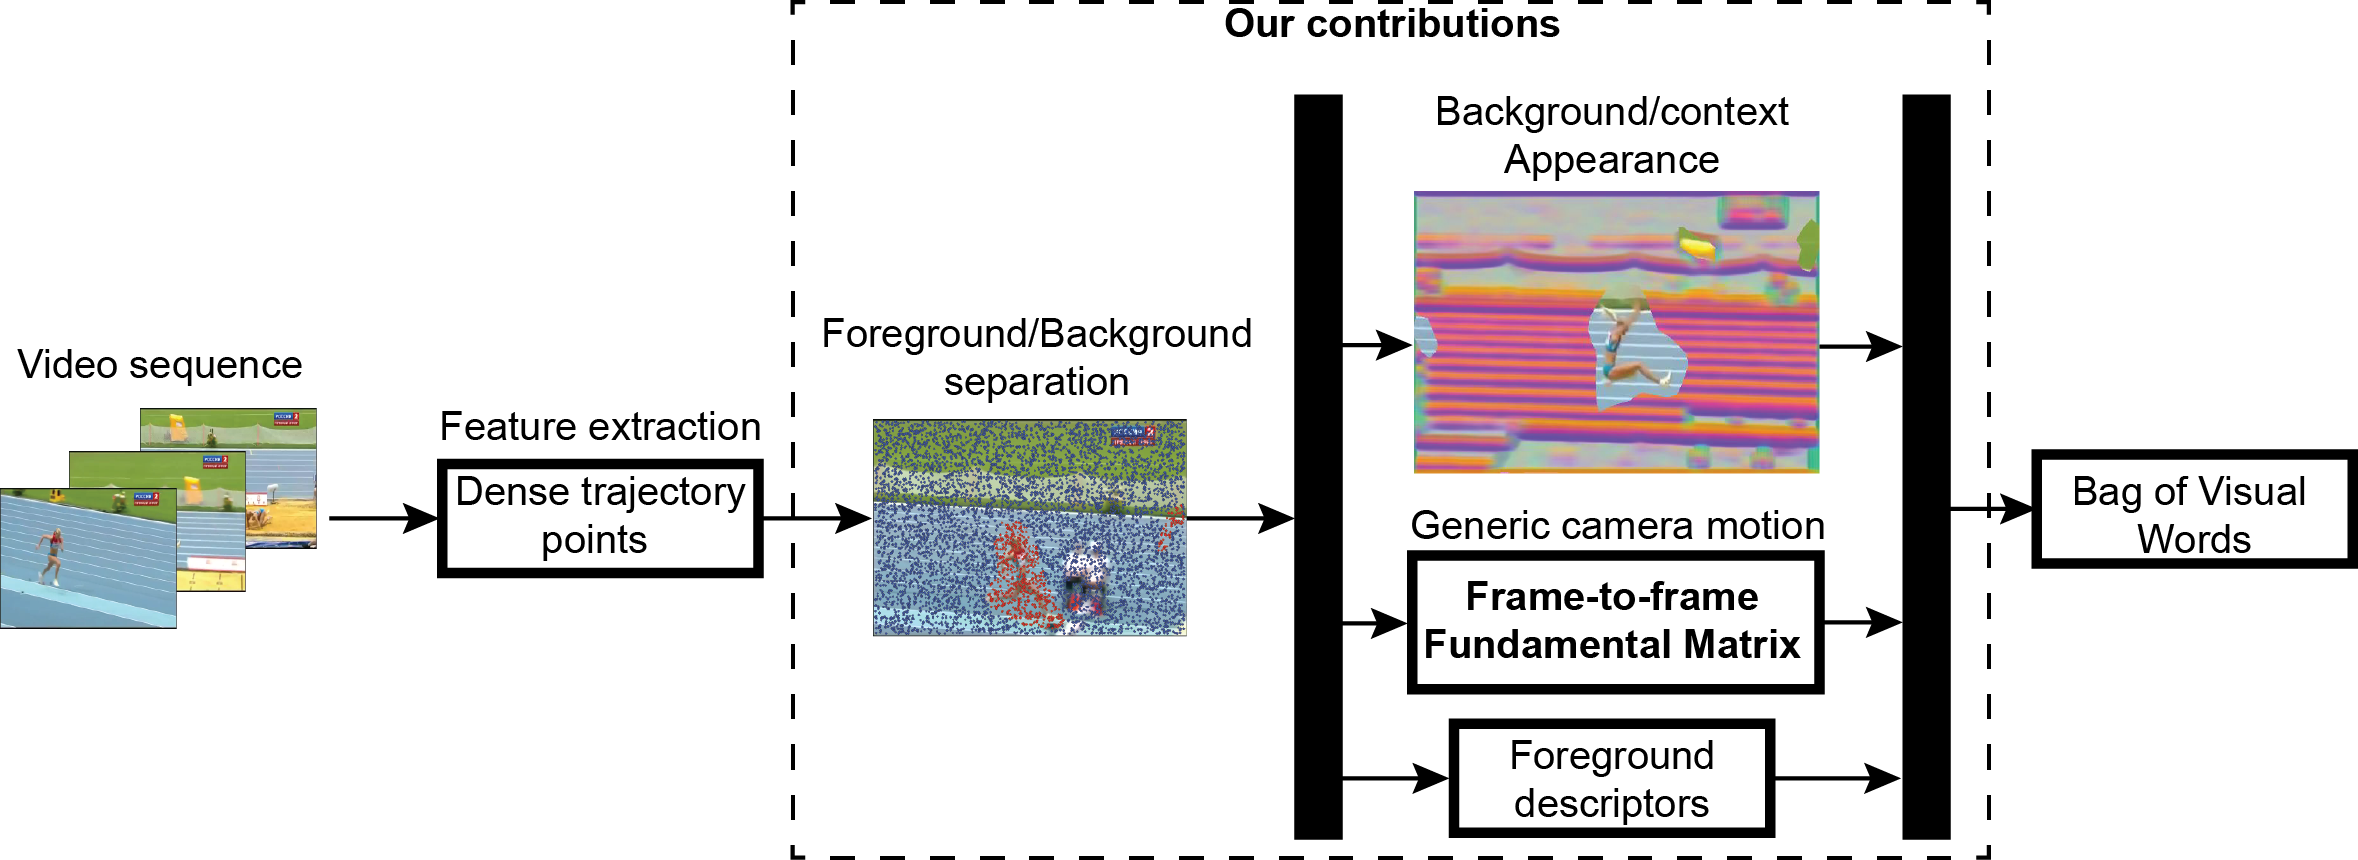
\includegraphics[width=0.98\linewidth]{pipeline.png}
\end{center}
\caption{Given a video sequence, a set of dense points trajectories are extracted. Then, a Fundamental Matrix is used for both applying a camera compensation and separating foreground/background trajectories. Each type of trajectories are encoded by different type of descriptors. Specifically, a low level global motion is used to generally describe the camera movement. Moreover, surrounding scene appearance is explicitly computed on background trajectories. Traditional foreground descriptors (\emph{e.g.} MBH, HOF, HOG and trajectory shape) are also aggregated in actions description. Finally, this set of descriptors are encoded separately using the BoF framework.}
\label{fig:pipeline}
\end{figure*}

This section gives a detailed description of our proposed approach for action recognition in video. The methodology in this paper follows the conventional action recognition pipeline. Given a set of labelled videos, a set of features is extracted from each video, represented using visual descriptors, and combined into a single video descriptor, which is used to train a multi-class classifier for recognition.

In this paper, we use dense point trajectories (short tracks of a densely sampled set of pixels in a video \cite{wang2013}) as our primitive features. By estimating frame-to-frame camera motion (fundamental matrix), we separate foreground trajectories corresponding to the action from background ones. Each type of trajectory is represented using a different descriptor. Foreground trajectories are represented using conventional visual properties (\emph{e.g.} MBH, HOF, HOG, and trajectory shape), while the surrounding scene appearance is described using SIFT. Foreground and background trajectories are then encoded separately using the BoF framework as illustrated in Figure \ref{fig:pipeline}. Unlike other action recognition methods, we not only use the frame-to-frame camera motion to separate foreground from background, but we also use it to \emph{describe} a video. This is done by encoding all frame-to-frame fundamental matrices in a video using the BoF framework. We use all three descriptors (foreground, surrounding scene appearance, and camera motion) to train a multi-class classifier for recognition. In this paper, we argue and show that combining a foreground-only description \cite{wang2013} with additional cues (background/context and camera motion) provides a richer and more discriminative description of actions.
%-------------------------------------------------------------------------
\subsection{Camera Movement}
\label{subsec:cam_motion}
Since videos are normally filmed with the intention of maintaining the subject within the image frame, there exists a relationship between the estimated camera movement and the underlying action. In this paper, we argue and show that this relationship can be a useful cue for discriminating certain action classes. As observed in the three top rows of Figure \ref{fig:camMotion_example}, there is a correlation between how camera moves and the subject, \emph{e.g.} in the second row, the \textit{cameraman} operates a till down in order to register the movement of the diver. Here, we do not claim that this cue is significant for all types of actions, since very similar camera motion can be shared among classes. Also, several actions not involves subjects translations, as noticed in Figure \ref{fig:camMotion_example} (\textbf{last two rows}). Instead of using a homography to encode camera motion, we estimate the more general fundamental matrix for each pair of frames in a video using the well-known 8-point algorithm \cite{eightpoint97}. As mentioned earlier, a homography is suitable to describe camera motion when the camera is not translating or when the background is planar; however, it is not applicable in more complex or cluttered scenes.

In our experiments, we calculate \textbf{camera motion descriptors} as follows. After estimating all pairwise fundamental matrices using RANSAC, we encode the camera motion of a video using the BoF framework. We call this descriptor CamMotion and it is complementary to other visual descriptors of the video. Unlike most existing work, we embrace camera motion and employ a low-level feature to capture this global motion in the video.
%-------------------------------------------------------------------------
\subsection{Surrounding Scene Appearance}
We now consider a camera compensation using our global motion model introduced in section \ref{subsec:cam_motion}. Exploiting the well performance of this compensation, we can easily separate trajectory points associated with the background, which tend to present a small displacement over the length of the trajectory. Taking advantage of this, we threshold trajectory displacement to obtain a foreground-background separation. The trajectory displacement is computed as follow:

\begin{equation}
D = \sum _{j=t}^{t+L-1}\left ( (x_{t+1}-x_t)^2, (y_{t+1}-y_t)^2 \right ).
\end{equation}

Trajectory points are associated with the background if $D<=\alpha$. Otherwise, those trajectory points are labeled as foreground. Empirically, we set this threshold value to $\alpha=3$ pixels.

Figure \ref{fig:approach} shows an example of our foreground-background separation in a video associated with the action \textit{long jump}. Here, foreground and background trajectories are color-coded in red and blue respectively. Clearly, the foreground trajectories correspond to the underlying action itself, while background trajectories correspond to \emph{static} background pixels undergoing camera motion only. Our proposed separation will allow each type of trajectory (foreground and background) to be represented independently and thus more reliably than other methods that encode context information using features from the entire frame \cite{marszalek2009}.

In practice, we calculate \textbf{foreground descriptors} that consist of Trajectory Shape, HOG, HOF, and MBH computed over dense trajectories as in \cite{wang2013}. In the following section, we detail how surrounding scene appearance is encoded.


\begin{figure*}[t!]
\begin{center}
%\fbox{\rule{0pt}{3in} \rule{0.9\linewidth}{0pt}}
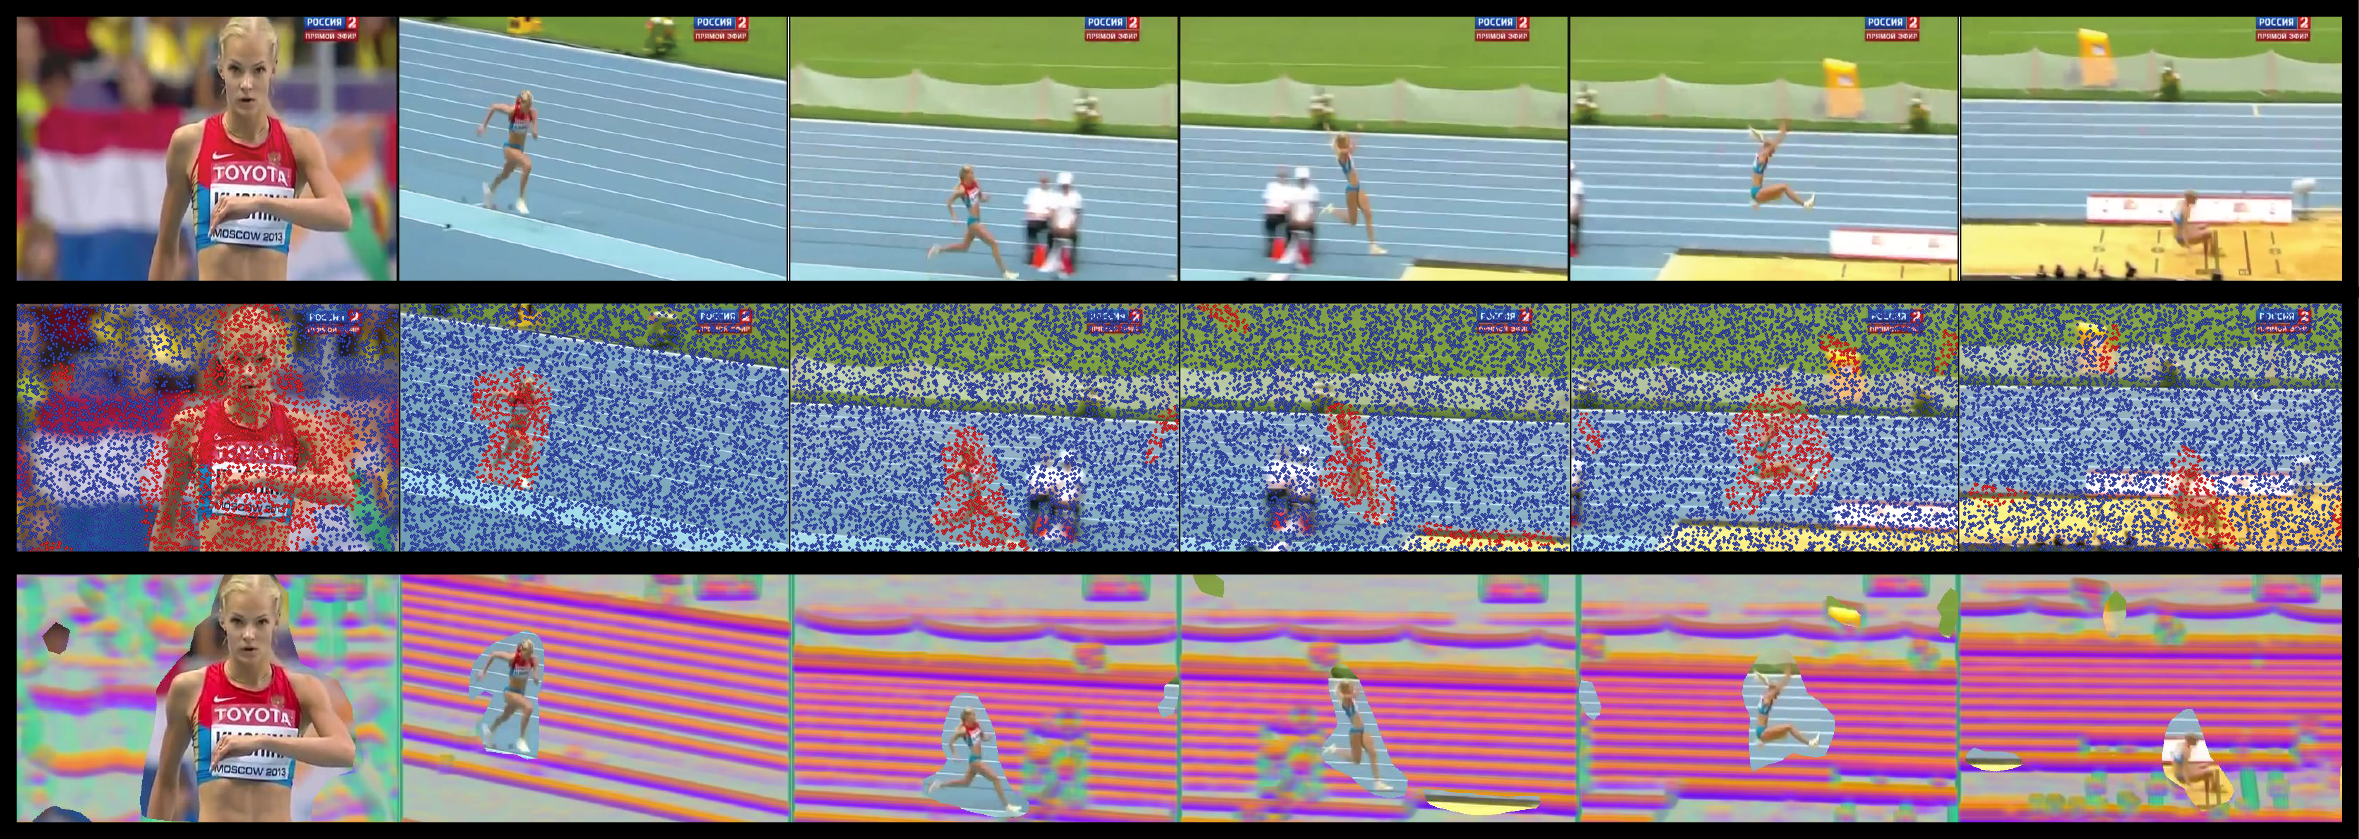
\includegraphics[width=0.98\linewidth]{approach.png}
\end{center}
\caption{Obtained results from our foreground-background separation and illustration of the encoded information by the surrounding scene features. \textbf{Top}. Frame sequence sampled from a long jump video. Note that camera is panning to follow the subject. \textbf{Middle}. Camera compensation allows to perform a background-foreground separation. Noticeably, foreground feature points are mostly related with the subject. \textbf{Bottom}. Illustration of information captured by our surrounding SIFT. In order to achieve a meaningful illustration, descriptor dimensionality is reduced to 3 dimensions to produce a color-coded image. As illustrated, surrounding appearance is captured only from pixels related with the scenario \emph{i.e.} avoiding pixels related to the subject that executes the action.}
\label{fig:approach}
\end{figure*}

%-------------------------------------------------------------------------

\subsection{Background/Context Appearance}
Human actions could be recognized by a set of cues. Beyond local motion and appearance properties of an action, the surrounding in which an action is performed is a critical component to recognize actions. For example, a 'springboard' action can only be executed if there is a pool, which has distinctive appearance properties. This motivates us to encode the visual appearance of the static scene. Surrounding scene appearance is encoded using SIFT descriptors \cite{lowe2004} around trajectory points associated with the background. We detect SIFT keypoints in a dense manner and then filter out those that fall within the union of foreground trajectories. Context appearance focuses more on the scenario itself, as observed in Figure \ref{fig:approach}. Additionally, in Figure \ref{fig:sift_example} is noticed how context appearance can be used to aggregate meaningful information about the action. For example, all presented thumbnails for the action rowing contains a shared landmark which can be exploited modeling the appearance of background points.  Unlike other methods that scene encode context holistically in a video \cite{marszalek2009}, separating the background/context from the foreground produces a more reliable and robust surrounding descriptor.

\begin{figure*}[t!]
\begin{center}
%\fbox{\rule{0pt}{3in} \rule{0.9\linewidth}{0pt}}
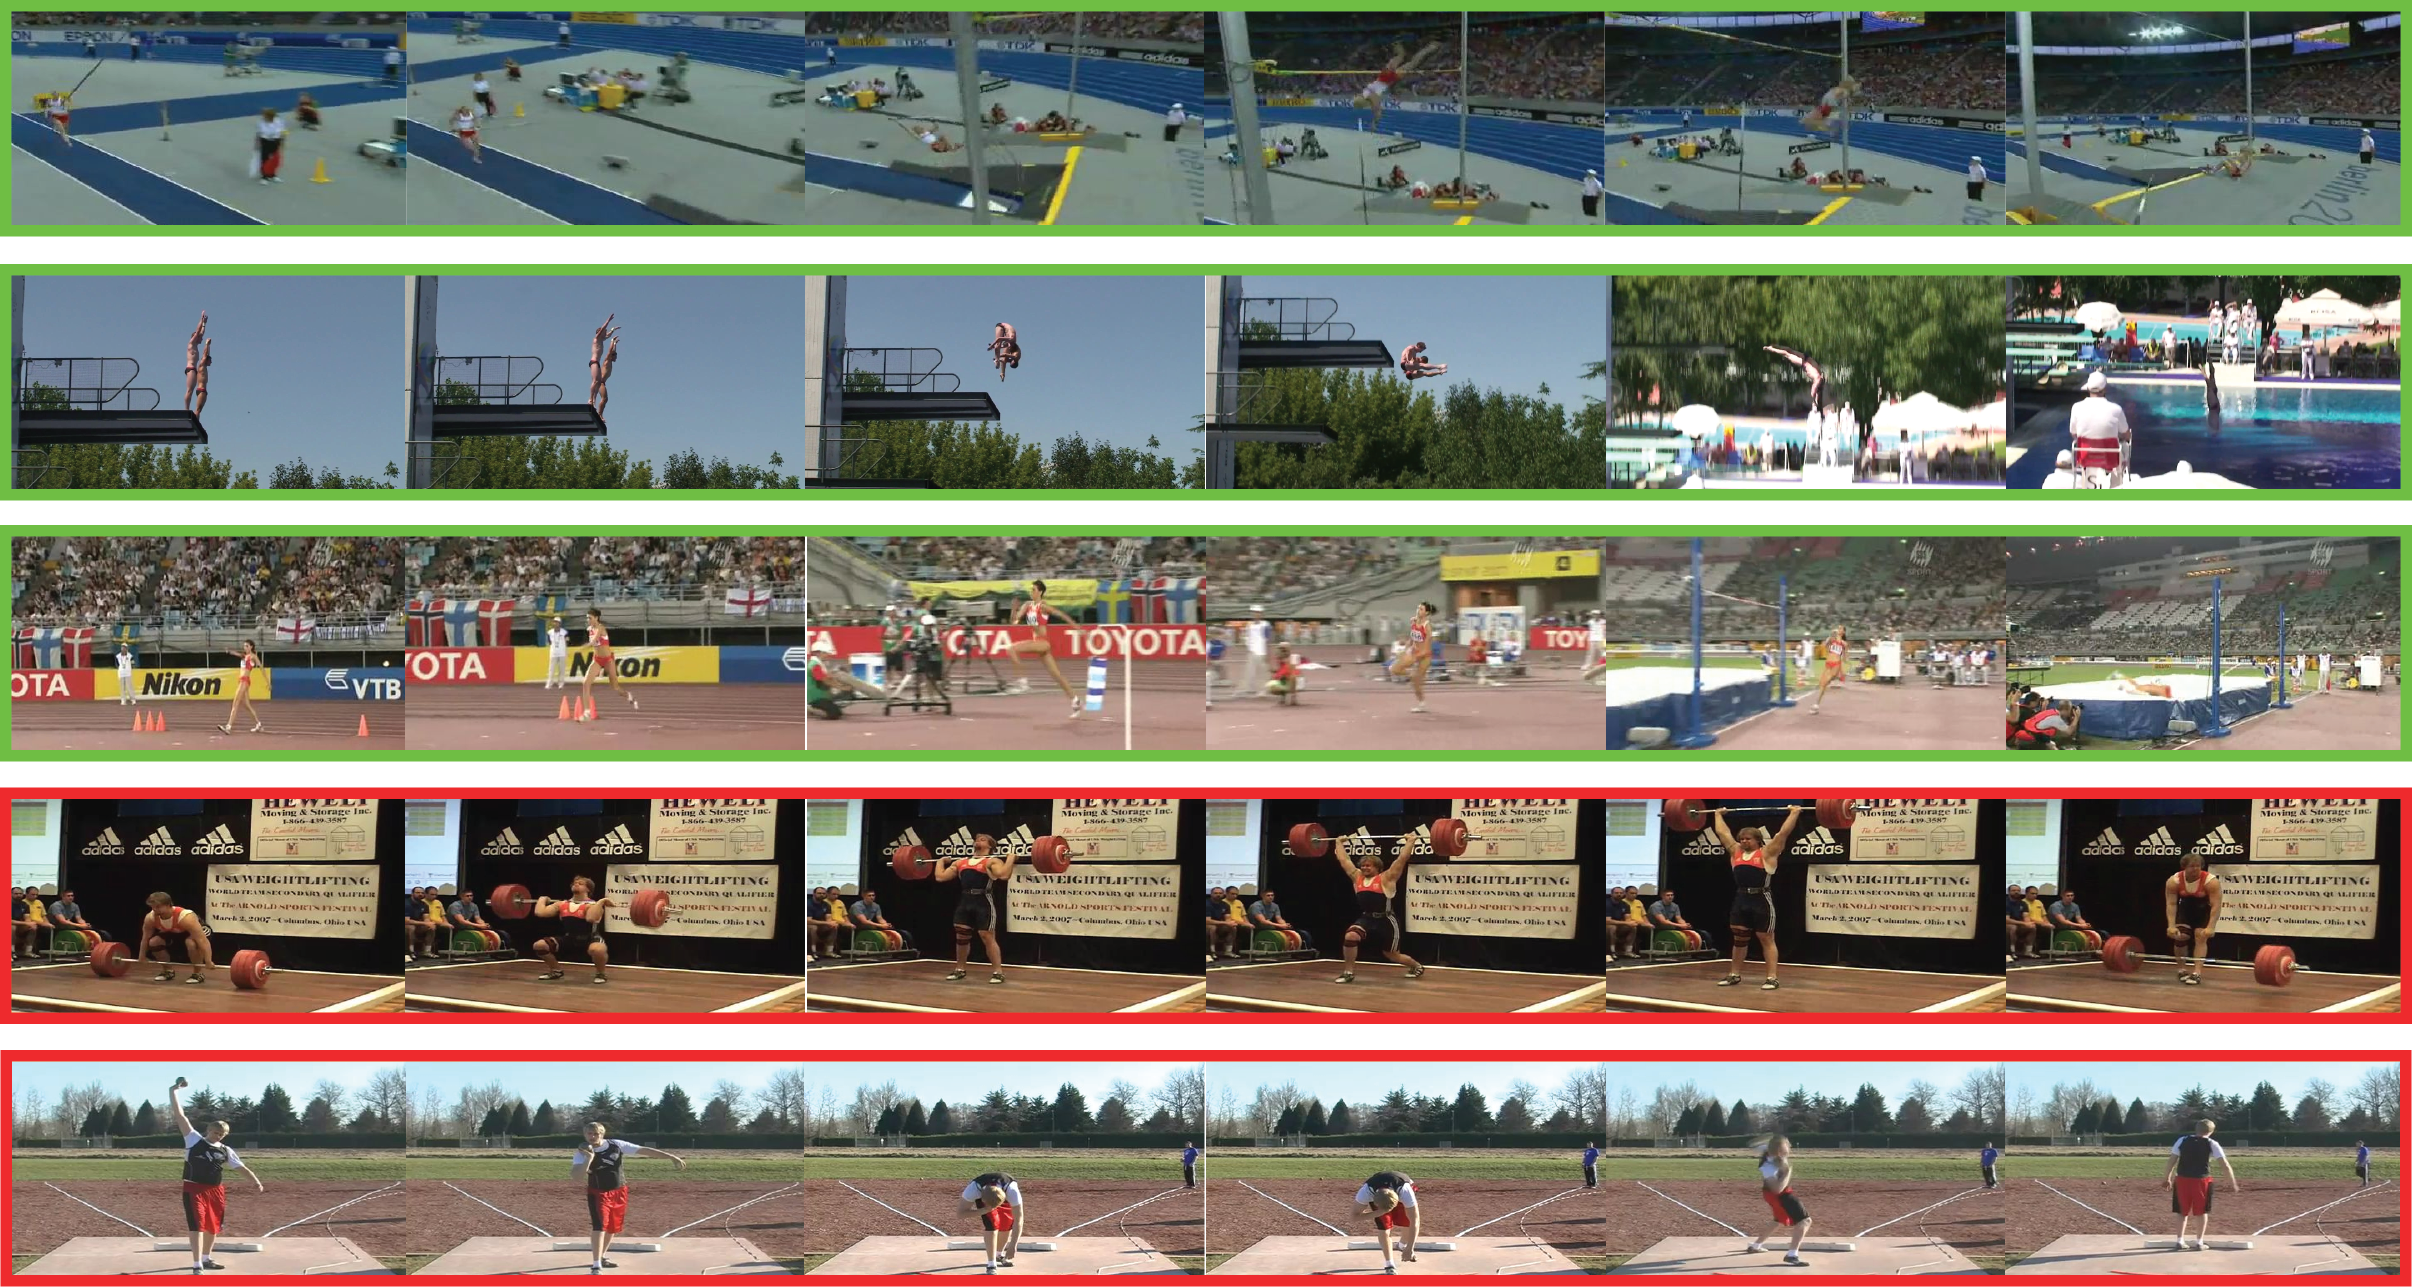
\includegraphics[width=0.98\linewidth]{cam_motion.png}
\end{center}
\caption{A generic camera motion descriptor can be a useful cue for discriminating specific action categories. As illustrated, the first three rows contains a characteristic correlation between how camera moves and the associated action. Unfortunately, this type of cue its not significant for all type of actions as shown in the last two rows where camera does not move at all.}
\label{fig:camMotion_example}
\end{figure*}

\begin{figure*}[t!]
\begin{center}
%\fbox{\rule{0pt}{3in} \rule{0.9\linewidth}{0pt}}
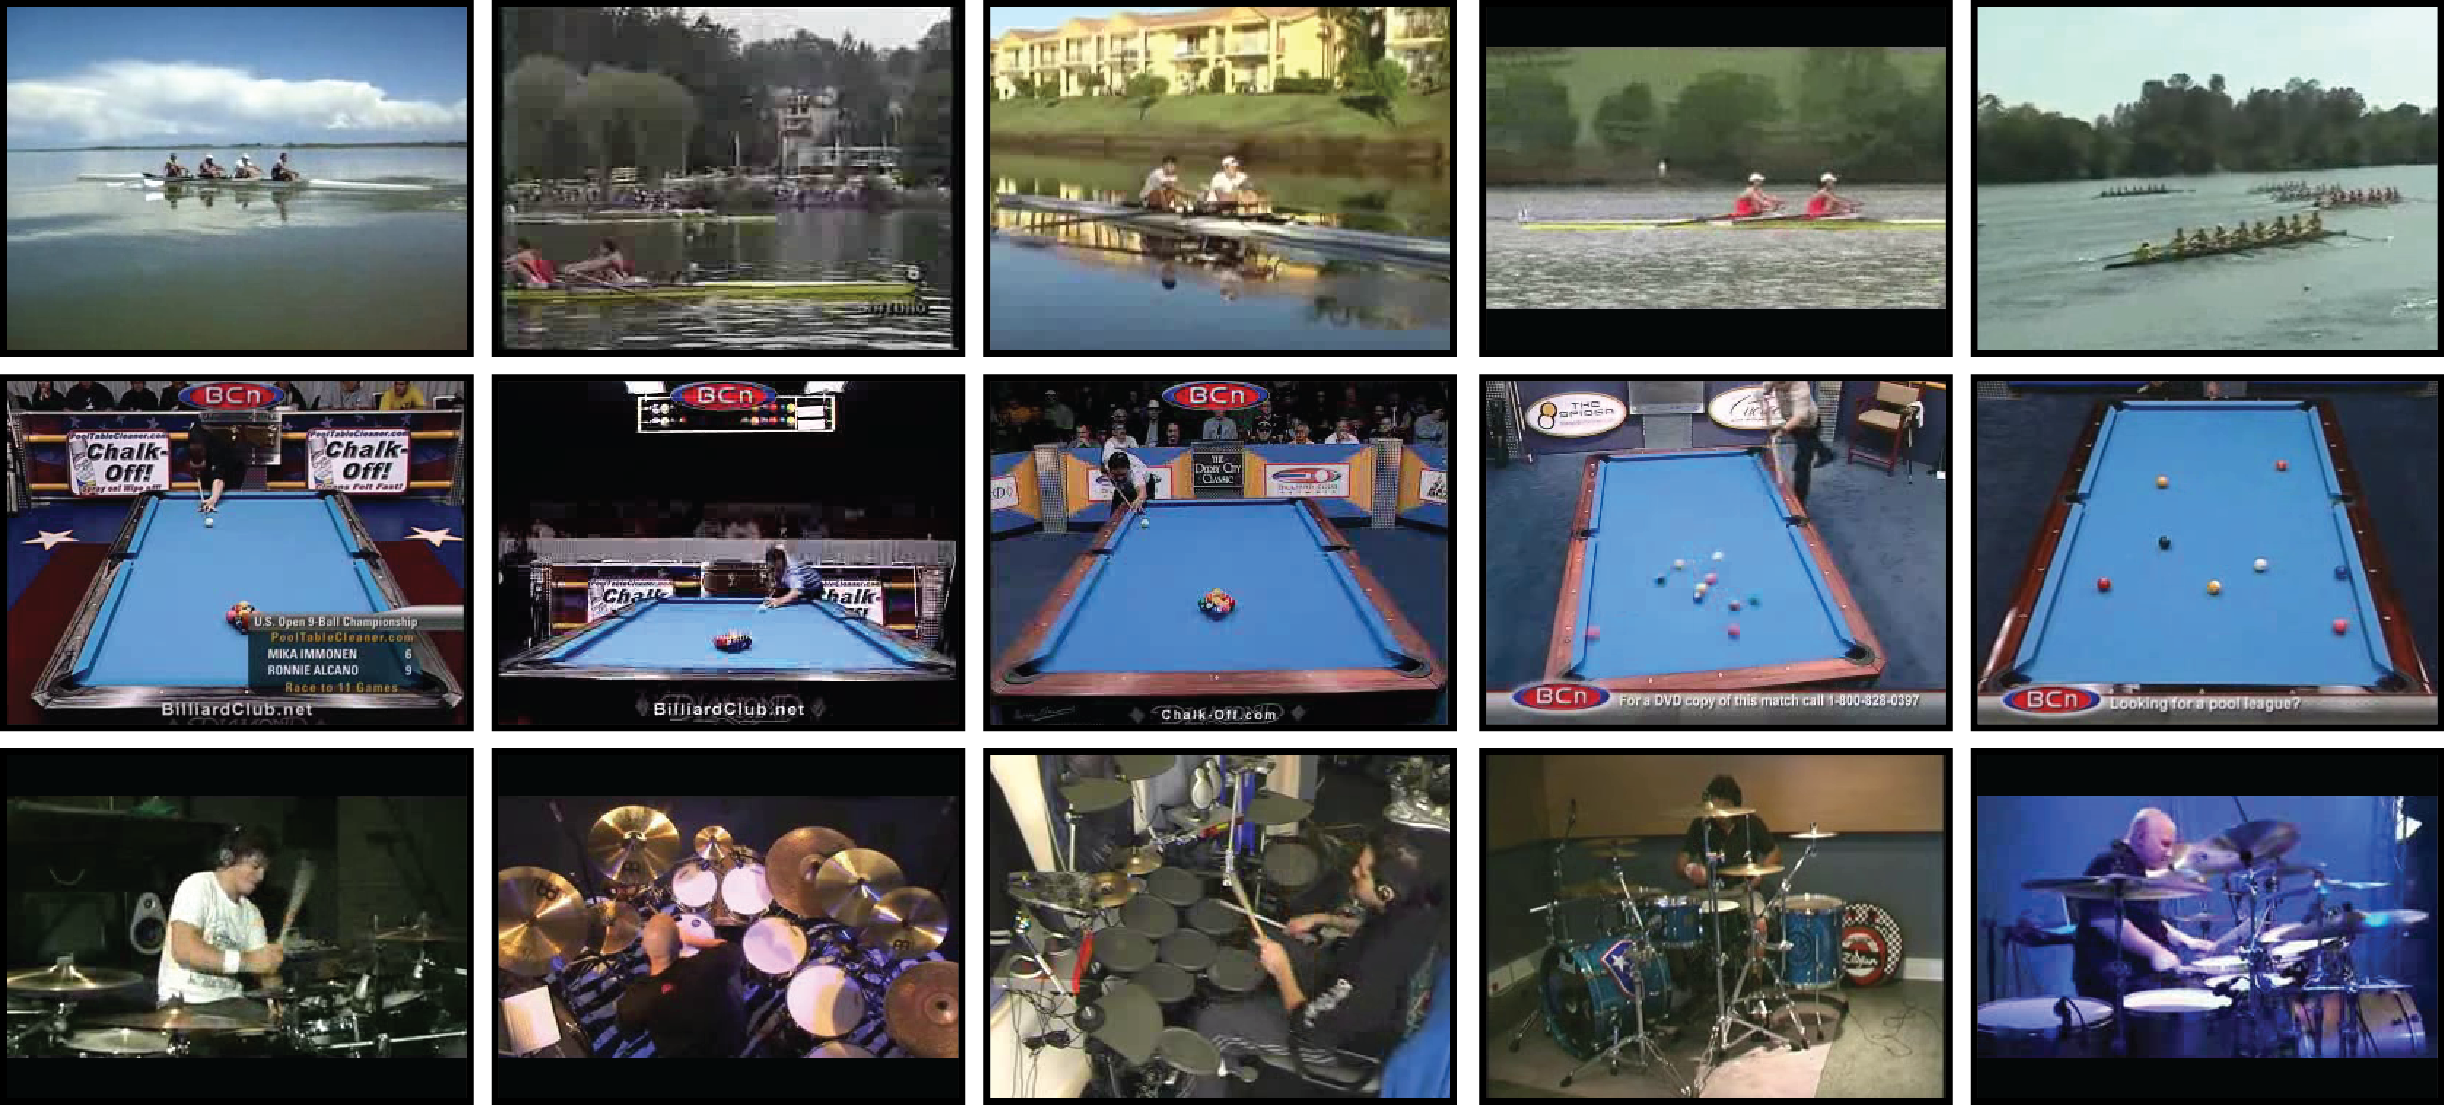
\includegraphics[width=0.98\linewidth]{sift.png}
\end{center}
\caption{Each row presents five different thumbnails taken from different videos of UCF50 dataset. \textbf{Top} row corresponds to examples of `rowing'. As observed all thumbnails share distinct background appearance \emph{i.e.} in all water is present and also in the majority there is a common landmark. In the \textbf{Middle} row, different billiard examples are depicted. A billiard table and the indoor environment of the action, enable our surrounding appearance descriptor to capture critical information about that action. Finally, \textbf{Bottom} row shows examples from the drumming category. Note that these examples share visual cues that are largely ignored if only foreground features are used.}
\label{fig:sift_example}
\end{figure*}

%-------------------------------------------------------------------------
\subsection{Implementation details}

\textbf{Codebook generation}. We generate the visual codebook in two different ways: (a) using \textbf{\textit{k}-means}, where we cluster the visual space, or, (b) using a \textbf{Gaussian Mixture Model (GMM)}, which captures a probability distribution over feature space. In both cases, a codebook is computed for each descriptor separately. Because of trajectory points methodologies produces a large amount of features resulting in intractable codebook computations, it is necessary to sub-sample the features extracted in the training examples for the purpose of codebook generation. In order to establish a trade-off between computation cost and recognition performance, we study the effect of the number of sampled features for computing a visual codebook, as observed in Figure \ref{fig:feature_sampling}. This experiment includes results in two different datasets using \textit{k}-means to form the visual dictionary. Additionally, we employ a spatial clustering sampling which shows a better performance compared to the uniform sampling. Mentioned spatial clustering finds K centers using \textit{k}-means over all features in a video. Then, the nearest trajectories on that centers are selected as the features to describe the video. In the following, we employ approximately 5 millions of feature points (~8GB RAM required per descriptor) sampled with a spatial clustering to form visual codebooks.\\\\
\textbf{Feature encoding} is performed under two different methodologies: (a) following the traditional histogram quantization (VQ), or, (b) applying the recently introduced Fisher vectors \cite{perronnin2010}. Different types of \textbf{Normalization} are performed to make feature vectors more robust: (a) \textit{l2} normalization (L2) \cite{perronnin2010}, (b) power normalization (PW) \cite{perronnin2010} and (c) intra-normalization (IN) \cite{xwang2013}. \\\\
\textbf{Framework representation}. We adopt two majors frameworks for action recognition. One of them follows the Bag of Features (BoF) paradigm, using \textit{k}-means for computing visual codebook, encoding features using VQ and L2 normalization, and finally learning action models with a non-linear SVM with $\chi^2$ kernel within a multichannel approach (MCSVM) as in \cite{zhang2007}:
\begin{equation}
K(x_i,x_j)= \exp(-\sum_c {\frac{1}{2\Omega_c} D_c(x_i,x_j)}),
\label{eq:multichannel}
\end{equation}
where $D_c(x_i,x_j)$ is the $\chi^2$ distance for channel $c$, and $\Omega_c$ is the average channel distance. Moreover, we implement a more robust framework (Fisher vectors) learning a codebook using a GMM. Consequently, we encode the feature vectors using the Fisher vectors. In this case, we apply three normalization strategies, L2, PW and IN as proposed in \cite{xwang2013}. Finally, normalized channels are concatenated and action models are learned within a linear SVM (LSVM). Described approaches are summarized in Table \ref{tab:frameworks}.

%%%%%%%%%%%%%%%%% Figure: Effect of sampling %%%%%%%%%%%%%%%%%%%
\begin{figure*}[t!]
\begin{center}
%\fbox{\rule{0pt}{1.2in} \rule{0.9\linewidth}{0pt}}
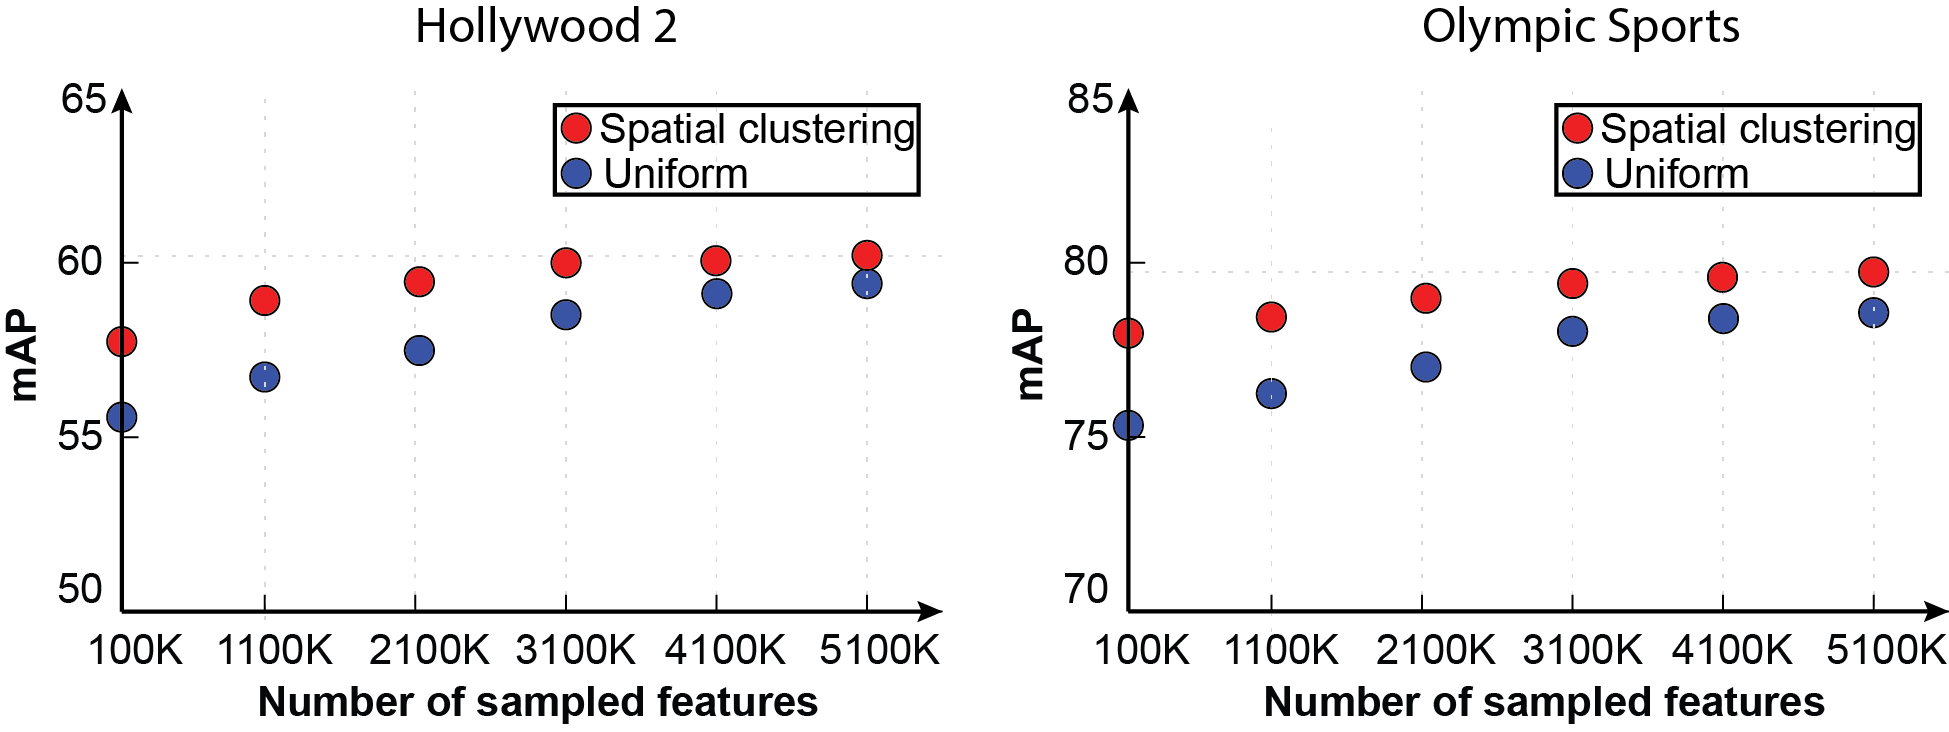
\includegraphics[width=0.98\linewidth]{sampling.png}
\end{center}
\caption{Due the extensive amount of features generated in a dense trajectory extraction approach, generally sub-sample is required to generate a codebook. Here, we explore the effect of the number of sampled features in the overall performance. Comparison is effectuated on two different datasets under the Bag of Features framework. Additionally, the effect in performance of two different sampling strategies are studied: uniform and spatial clustering. As noticed, selecting more features to form the codebook and using the spatial clustering sampling benefit recognition performance in both datasets evaluated.}
\label{fig:feature_sampling}
\end{figure*}
%%%%%%%%%%%%%%%%%%%%%%%%%%%%%%%%%%%%%%%%%%%%%%%%%%%%%%%%%%%%%%%%


%%%%%%%%%%%%%%% Table: Frameworks comparison %%%%%%%%%%%%%%%%%%%
\begin{table*}[h!]
\caption{Comparison of adopted frameworks for action recognition.}
\begin{center}
{
\begin{tabular}{ l| c c c c c }
\hline
Representation $\downarrow$ & Codebook & Encoding & Normalization & Classifier \\
\hline
Bag of Features & \textit{k}-means & VQ & L2 & MCSVM \\
Fisher vectors & GMM & Fisher vectors & L2+PW+IN & LSVM \\
\hline
\end{tabular}
}
\end{center}
\label{tab:frameworks}
\end{table*}
%%%%%%%%%%%%%%%%%%%%%%%%%%%%%%%%%%%%%%%%%%%%%%%%%%%%%%%%%%%%%%%%

%===========================================================
\section{Experimental results}
\label{results}
\subsection{Datasets and evaluation protocol}
\label{subsec:datasets}
We use four public datasets \cite{kuehne2011, marszalek2009, niebles2010, reddy2013} and their corresponding evaluation protocols. In this section we briefly describe each dataset.

\textbf{HMDB51} \cite{kuehne2011} includes a large collection of human activities categorized on 51 classes. It collects 6766 videos from different media resources \emph{i.e.} digitized movies, public databases and user generated web video data. Due to a large amount of videos contains undesired camera motions, the authors provide a stabilized version of the dataset. However, since we look at the camera motion as an informative cue, non-stabilized version of the dataset is used. For evaluating performance, we adopt the same protocol proposed by the dataset authors \emph{i.e.} computing the mean accuracy under three fixed train/test splits.

\textbf{Hollywood2} \cite{marszalek2009} contains a wide number of videos retrieved from 69 different Hollywood movies. It is divided in 12 categories including short actions such as Kiss, Answer Phone and Stand Up. This dataset remains as one of the most challenging despite the small number of action classes. Change of camera view,  camera motion and unchoreographed execution introduces more difficult a the time of recognition. To evaluate performance, we follow the author's protocol where videos are separated in two different sets: a training set of 823 videos and a testing set of 884 videos. We use training videos to learn our action models and then compute the mean average precision (mAP) over all action classes.

\textbf{Olympic Sports} \cite{niebles2010} or \textbf\textit{{Olympic}} comprises a set of 783 sport related YouTube videos. This set of videos are semi-automatically labeled using Amazon Mechanical Turk. This dataset establish new challenges for recognition because of it jumps from simple actions (\emph{e.g.} Kiss) to complex actions (\emph{e.g.} Hammer throw). All of these complex actions are related with olympic sports including actions like \textit{Long jump}, \textit{Pole vault} and \textit{Javelin throw}. As proposed by the author's dataset, we measure performance calculating the mAP over all dataset categories.

\textbf{UCF50} \cite{reddy2013} includes 6618 videos of 50 different human actions.  This dataset presents several recognition challenges due to large variations in camera motion, cluttered background, viewpoint, etc. Action categories are grouped into 25 sets, where each set consists of more than 4 action clips. Recognition performance is measured by applying a leave-one-group-out cross-validation and average accuracy over all group splits is reported.

%-----------------------------------------------------------
\subsection{Impact of contextual features}
We conduct further experiments to measure the  contribution of our proposed camera movement (CamMotion) and surrounding scene appearance descriptor (SIFT). Our Baseline corresponds to using only Foreground features for describing actions. Per-descriptor performances are compared to that established baseline. Also, we investigate the effect of combining proposed features with Foreground cues. As well, CamMotion and SIFT performance is evaluated under two action recognition representations \emph{i.e.} Bag of Features and Fisher vectors. Below, we present an analysis of obtained results.\\\\
\textbf{Representation}. As suggested in recent works \cite{perronnin2010, wang2013, xwang2013} Fisher vectors provides a boosted performance compared to traditional Bag of Feature representations. We found in our experiments that Fisher vectors also boost our contextual descriptors performance, as presented in Table \ref{tab:features}. However, we note that using Fisher vectors is less important with our CamMotion descriptor due to its low dimensionality. Even so, Fisher vectors are used for following analysis.\\\\
\textbf{Foreground-background}. As described in Section \ref{scene}, we perform a weak separation between background and foreground feature points. We measure the effect on performance of this separation in proposed features. We note that this type of weak segmentation provides a significant boost in performance, as observed in Table \ref{tab:segmentation}. When feature points are localized on the background, surrounding SIFT focuses on the scene appearance avoiding information of actors and foreground objects. The gain of surrounding SIFT over all the holistic approach is as follow: +0.3\% for HMDB51, +4.2\% for Hollywood2, +5.2\% for Olympics and +3.9\% for UCF50. The same behavior is observed with our CamMotion descriptor where performance is boosted in all datasets due to Fundamental Matrix is computed based on background tracks.\\\\
\textbf{Surrounding appearance}. While by itself SIFT achieves a discrete performance, it produces notable improvements when combined with foreground descriptors. As Table \ref{tab:features} reports, performance is significantly improved over all datasets. Interestingly, we note that surrounding SIFT produces higher improvements in HMDB51 and UCF50 \emph{i.e.} +2.7\% and +2.4\% respectively.\\\\
\textbf{Camera movement}. Experiment results evidences that action recognition is noticeably improved when a global motion is incorporated to Foreground features. Our CamMotion provides slightly lower contributions in performance than the SIFT descriptor. We observe a significantly contribution over all datasets except on HMDB51 where recognition performance decrease. This negative effect is attributed to the extensive shared shaky camera in video sequences for this dataset. This unable our CamMotion to capture discriminative cues over action categories. 

%%%%%%%%%%%%% Table: Effect of selected points %%%%%%%%%%%%%
\begin{table*}[ht!]
\caption{Effect of separating background feature points surrounding SIFT and CamMotion. Experimental results consistently show that SIFT exhibit better results when is capturing the surrounding appearance of actions. Conversely, CamMotion and SIFT tend to be more discriminative when computed in non-foreground feature points.}
\begin{center}
{
\begin{tabular}{|c|c c|c c c c|}
\hline
& \multicolumn{2}{|c|}{Feature points} & \multicolumn{4}{|c|}{Datasets} \\
Feature $\downarrow$ & Foreground & Background & HMDB51 & Hollywood2 & Olympics & UCF50 \\
\hline
SIFT & \checkmark & & 19.5\% & 22.1\% & 33.5\% & 44.7\% \\
SIFT & & \checkmark & \textbf{20.1\%} & \textbf{28.5\%} & \textbf{39.6\%} & \textbf{49.8\%} \\
SIFT & \checkmark & \checkmark & 19.8\% & 24.3\% & 34.4\% & 45.9\% \\
\hline
CamMotion & \checkmark & & 9.7\% & 14.9\% & 19.5\% & 13.7\% \\
CamMotion & & \checkmark & \textbf{14.1\%} & \textbf{22.1\%} & \textbf{27.2\%} & \textbf{19.5\%} \\
CamMotion & \checkmark & \checkmark & 12.9\% & 18.7\% & 21.8\% & 17.2\% \\
\hline
\end{tabular}
}
\end{center}
\label{tab:segmentation}
\end{table*}
%%%%%%%%%%%%%%%%%%%%%%%%%%%%%%%%%%%%%%%%%%%%%%%%%%%%%%%%%%%%

%%%%%%%%%%%%%% Table: Feature analysis %%%%%%%%%%%%%%%%%%%%%
\begin{table*}[ht!]
\caption{Impact of our surrounding scene appearance and camera movement in recognition performance. Bag of Features generally performs poor than Fisher vectors. Both surrounding SIFT and CamMotion show important improvements in performance when they are combined with foreground descriptors.}
\begin{center}
{
\def\arraystretch{1.11}
\setlength{\tabcolsep}{3.66pt}
\begin{tabular}{ |c c c|c c c c| }
\hline
\multicolumn{3}{|c|}{Features} & \multicolumn{4}{|c|}{Datasets} \\
Foreground & SIFT & CamMotion & HMDB51 & Hollywood2 & Olympics & UCF50 \\
\hline
\multicolumn{7}{|c|}{Framework: Bag of Features} \\
\hline
\checkmark & & & 51.2\% & 60.1\% & 79.8\% & 85.9\% \\
& \checkmark & & 19.5\% & 28.7\% & 36.4\% & 45.7\% \\
& & \checkmark & 13.5\% & 21.8\% & 26.9\% & 19.3\% \\
\checkmark & \checkmark & & 53.8\% & 60.9\% & 81.1\% & 87.2\% \\
\checkmark &  & \checkmark & 50.9\% & 60.4\% & 80.6\% & 86.8\% \\
& \checkmark & \checkmark & 20.7\% & 36.2\% & 43.7\% & 50.3\% \\
\checkmark & \checkmark & \checkmark & 51.7\% & 61.6\% & 81.7\% & 87.6\% \\
\hline
\multicolumn{7}{|c|}{Framework: Fisher vectors} \\
\hline
\checkmark & & & 56.5\% & 62.4\% & 90.4\% & 90.9\% \\
& \checkmark & & 20.1\% & 28.5\% & 39.6\% & 49.8\% \\
& & \checkmark & 14.1\% & 22.1\% & 27.2\% & 19.5\% \\
\checkmark & \checkmark & & \textbf{59.2\%} & \textbf{63.5\%} & \textbf{91.6\%} & \textbf{93.3\%} \\
\checkmark &  & \checkmark & 55.9\% & 62.9\% & 91.3\% & 93.1\% \\
& \checkmark & \checkmark & 22.3\% & 36.5\% & 46.5\% & 54.3\% \\
\checkmark & \checkmark & \checkmark & \textbf{57.9\%} & \textbf{64.1\%} & \textbf{92.5\%} & \textbf{93.8\%} \\
\hline
\end{tabular}
}
\end{center}
\label{tab:features}
\end{table*}

%-----------------------------------------------------------
\subsection{Comparison with the state of the art}
We set side by side our method with recent methods that address the same application using similar representations, \emph{i.e.} methods that use dense trajectory points to represent video sequences \cite{wang2013, jiang2012, jain2013} in Table \ref{tab:stateofart}. We also present results for our own implementation of \cite{wang2013}, which correspond to our baseline (Foreground). The gain over the recent paper \cite{wang2013}, which reports the best performance in the literature, is as follow: \textbf{+2\%} for HMDB51, \textbf{+1.4\%} for Olympic Sports and \textbf{2.6\%} for UCF50. We also achieve a comparable performance on Hollywood2 dataset with only 0.2\% less in the mAP value. Since Human Detection (HD) is not included in our trajectory extraction stage, a more direct comparison its the non-HD approach of Wang \emph{et al.} \cite{wang2013}. In that case, our method outperforms their improved trajectories in \textbf{3.3\%} for HMDB51, \textbf{1.1\%} for Hollywood2, \textbf{2.3\%} for Olympic Sports and \textbf{3.3\%} for UCF50.

%%%%%%%%%%%%%% Table: State-of-the-art %%%%%%%%%%%%%%%%%%%%%%
\begin{table*}[ht!]
\caption{Comparison with the state-of-the-art on challenging datasets. Our method improves reported results in the state-of-the-art for three different datasets, HMDB51, Olympic Sports and UCF50 and obtains competitive peformance in Hollywod2.}
\begin{center}
{
\begin{tabular}{ |l| c c c c| }
\hline
Approach $\downarrow$ & HMDB51 & Hollywood2 & Olympics & UCF50 \\
\hline
Jiang \emph{et al.} \cite{jiang2012} & 40.7\% & 59.5\% & 80.6 & - \\
Jain \emph{et al.} \cite{jain2013} & 52.1\% & 62.5\% & 83.2 & - \\
Wang \emph{et al.} \cite{wang2013} non-HD & 55.9\% & 63.0\% & 90.2\% & 90.5\% \\
Wang \emph{et al.} \cite{wang2013} HD & 57.2\% & \textbf{64.3\%} & 91.1\% & 91.2\% \\
\hline
\multicolumn{5}{|c|}{\textit{Our methods with Fisher vectors}} \\
\hline
Baseline (Foreground) & 56.5\% & 62.4\% & 90.4\% & 90.9\% \\
Foreground + SIFT & \textbf{59.2\%} & 63.5\% & \textbf{91.6\%} & \textbf{93.3\%} \\
Foreground + SIFT + CamMotion  & \textbf{57.9\%} & \textbf{64.1\%} & \textbf{92.5\%} & \textbf{93.8\%} \\
\hline
\end{tabular}
}
\end{center}
\label{tab:stateofart}
\end{table*}
%%%%%%%%%%%%%%%%%%%%%%%%%%%%%%%%%%%%%%%%%%%%%%%%%%%%%%%%%%%%%

\vspace{3mm}
\noindent {\bf Acknowledgment}. Research reported in this publication was supported by competitive research funding from King Abdullah University of Science and Technology (KAUST). F.C.H. is supported by a COLCIENCIAS Young  Scientist and Innovator Fellowship. J.C.N. is supported by a Microsoft Research Faculty Fellowship. 

%===========================================================
\bibliographystyle{splncs}

\begin{thebibliography}{10}

\bibitem{laptev2005}
Laptev, I.:
\newblock On space-time interest points.
\newblock IJCV (2005)

\bibitem{dollar2005}
Dollar, P., Rabaud, V., Cottrell, G., Belongie, S.:
\newblock Behavior recognition via sparse spatio-temporal features.
\newblock In: Visual Surveillance and Performance Evaluation of Tracking and
  Surveillance, 2005. (2005)

\bibitem{wang2011}
Wang, H., Klaser, A., Schmid, C., Liu, C.L.:
\newblock Action recognition by dense trajectories.
\newblock In: CVPR. (2011)

\bibitem{laptev2008}
Laptev, I., Marszalek, M., Schmid, C., Rozenfeld, B.:
\newblock Learning realistic human actions from movies.
\newblock In: CVPR. (2008)

\bibitem{blank2005}
Blank, M., Gorelick, L., Shechtman, E., Irani, M., Basri, R.:
\newblock Actions as space-time shapes.
\newblock In: ICCV. (2005)

\bibitem{schuldt2004}
Schuldt, C., Laptev, I., Caputo, B.:
\newblock Recognizing human actions: a local svm approach.
\newblock In: ICPR. (2004)

\bibitem{kuehne2011}
Kuehne, H., Jhuang, H., Garrote, E., Poggio, T., Serre, T.:
\newblock Hmdb: a large video database for human motion recognition.
\newblock In: ICCV. (2011)

\bibitem{marszalek2009}
Marszalek, M., Laptev, I., Schmid, C.:
\newblock Actions in context.
\newblock In: CVPR. (2009)

\bibitem{wang2013}
Wang, H., Schmid, C.:
\newblock Action recognition with improved trajectories.
\newblock In: ICCV. (2013)

\bibitem{aggarwal2011}
Aggarwal, J., Ryoo, M.S.:
\newblock Human activity analysis: A review.
\newblock ACM Computing Surveys (CSUR) (2011)

\bibitem{perronnin2010}
Perronnin, F., S{\'a}nchez, J., Mensink, T.:
\newblock Improving the fisher kernel for large-scale image classification.
\newblock In: ECCV.
\newblock (2010)

\bibitem{jegou2012}
J{\'e}gou, H., Perronnin, F., Douze, M., S{\'a}nchez, J., P{\'e}rez, P.,
  Schmid, C.:
\newblock Aggregating local image descriptors into compact codes.
\newblock PAMI (2012)

\bibitem{xwang2013}
Wang, X., Wang, L., Qiao, Y.:
\newblock A comparative study of encoding, pooling and normalization methods
  for action recognition.
\newblock In: ACCV.
\newblock (2012)

\bibitem{wu2011}
Wu, S., Oreifej, O., Shah, M.:
\newblock Action recognition in videos acquired by a moving camera using motion
  decomposition of lagrangian particle trajectories.
\newblock In: ICCV. (2011)

\bibitem{park2013}
Park, D., Zitnick, C.L., Ramanan, D., Doll{\'a}r, P.:
\newblock Exploring weak stabilization for motion feature extraction.
\newblock In: CVPR. (2013)

\bibitem{jain2013}
Jain, M., J{\'e}gou, H., Bouthemy, P.:
\newblock Better exploiting motion for better action recognition.
\newblock In: CVPR. (2013)

\bibitem{ikizler2010}
Ikizler-Cinbis, N., Sclaroff, S.:
\newblock Object, scene and actions: Combining multiple features for human
  action recognition.
\newblock In: ECCV.
\newblock (2010)

\bibitem{oliva2001}
Oliva, A., Torralba, A.:
\newblock Modeling the shape of the scene: A holistic representation of the
  spatial envelope.
\newblock IJCV (2001)

\bibitem{eightpoint97}
Hartley, R.:
\newblock In defense of the eight-point algorithm.
\newblock TPAMI (1997)  580--593

\bibitem{lowe2004}
Lowe, D.G.:
\newblock Distinctive image features from scale-invariant keypoints.
\newblock IJCV (2004)

\bibitem{zhang2007}
Zhang, J., Marsza{\l}ek, M., Lazebnik, S., Schmid, C.:
\newblock Local features and kernels for classification of texture and object
  categories: A comprehensive study.
\newblock IJCV (2007)

\bibitem{escorcia2013}
Niebles, J.C., Escorcia, V.:
\newblock Spatio-temporal Human-Object Interactions for Action Recognition in Videos
\newblock In: ICCV.
\newblock (2013)

\bibitem{niebles2010}
Niebles, J.C., Chen, C.W., Fei-Fei, L.:
\newblock Modeling temporal structure of decomposable motion segments for
  activity classification.
\newblock In: ECCV.
\newblock (2010)

\bibitem{reddy2013}
Reddy, K.K., Shah, M.:
\newblock Recognizing 50 human action categories of web videos.
\newblock Machine Vision and Applications (2013)

\bibitem{jiang2012}
Jiang, Y.G., Dai, Q., Xue, X., Liu, W., Ngo, C.W.:
\newblock Trajectory-based modeling of human actions with motion reference
  points.
\newblock In: ECCV.
\newblock (2012)

\end{thebibliography}

%this would normally be the end of your paper, but you may also have an appendix
%within the given limit of number of pages
%\end{document}

%===========================================================

\end{document}
